\section{Related work}
\begin{figure*}[htbp]
	\centering
	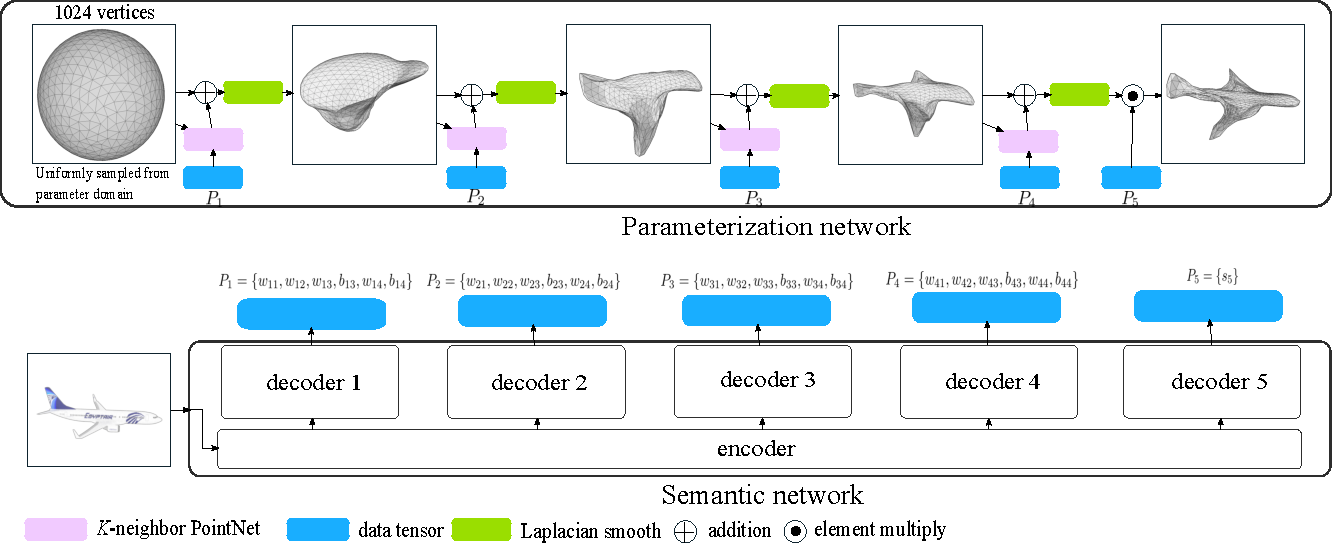
\includegraphics[width=\linewidth]{img/net/overview}
	\caption{The overview of the network: The proposed framework consists of two networks. One is the parameterization network that maps points sampled from parameter domain to target shape. The other is the semantic network that takes image as input and predict parameters for the parameterization network.}
	\label{fig:overview}
\end{figure*}
3D reconstruction/modeling from image have been 
 Especially, with the release of large-scale 3D shape datasets such as ShapeNet\cite{shapenetdata}, deep learning based approaches have achieved great progress.
 
\subsection{General learning approaches}
As far as we known, early works of learning approaches can be traced back to \cite{Hoiem2007} and \cite{learn3D2007}. More recent works like \cite{Su:2014} and \cite{jointimgshape} break down the problem to two stages, one is to retrieve shape components from a large dataset, the other is to assemble the components and deform the assembled shape to fit the observed image. However, shape retrieval from images itself
is an ill-posed problem due to the loss of information in 3D-to-2D projection. To avoid such problem, \cite{imgrecon15} propose a solution that start reconstruction from a learned 3D deformable shape. 
In \cite{imgrecon15}, images specify the shape variations and drive the shape deformation to target.

These learning approaches are relatively early. For their systems to work, complicate pre-process on database are usually needed. A more ideal solution would be to directly learn 3D shapes
from single images under an end-to-end framework. 

\subsection{3D neural networks}
Most recently, researchers have developed techniques to represent 3D shapes inside deep learning framework and developed a serious of 3D neural networks to predict 3D shapes from images. Unlike images, 3D shapes are not canonical functions. This leads to multiple exploration for their representation. Therefore, we group these works according to their 3D representation.

\noindent\textbf{Volume occupancy}
An intuitive way to extend the success of convolution network to 3D is to use volume occupancy of regular 3D grid to represent 3D shapes. Such 3D convolution was introduced by \cite{3dshapenet} and widely used in many works \cite{3DR2N2,learnobj} for 3D shape generation.

The key disadvantage of such representation was the large memory consumption due to the raising of dimension when extend 2D grid to 3D. The most recent work of \cite{octreegen} use
an octree representation for shape generation (similar representation is used in for 3D shape classification and segmentation by \cite{ocnn}), which allows to higher resolution outputs
with limited memory.

\noindent\textbf{Point cloud}
\cite{PSGN} proposed neural networks that regress unordered
3D point set for 3D shape generation. The point cloud representation
do not consider local connections of the points, and thus the point positions have
a very large degree of freedom. Consequently, it is difficult to reconstruct continue surface from the generated point cloud.

Besides the problem of generation/reconstruction, techniques like \cite{PointNet,NIPS2017_7095,pointcnn} have been developed so that the network can take unordered 3D point set as input and extract geometric features from 3D point set.

\noindent\textbf{Mesh}
Among all three representations, mesh is the most popular one in game and movie industries. In addtion to the vertex positions , the mesh representation also consider local structure of vertices. It is non-trivial to use mesh representation for 3D shape with end-to-end trainable neural networks. \cite{img2mesh} and \cite{endface} produce mesh by linear interpolating base meshes. Since it is only possible to choose/learn base meshes for specific class of object, these two networks can only generate mesh for specific class of object (the latter one is only used for human face).

\cite{3Drender} aims to make a differentiable approximation for 3D mesh rendering process, which would be much more significant if it can actually render gray image. In fact, the approximated renderer can only produce silhouette as output. When the it is used with mesh generation network, it can only take silhouette as supervision and hence does not perform well for complicated objects (car, airplane, etc.)

Our network produce mesh as output, but it draws a lot of experience from techniques designed for point cloud representation.

\subsection{Parameterization in learning approaches}
 The idea that utilize parameterization in the representation of 3D shape have been explored by the works of \cite{surfnet,geoimg}. These methods involves a non-trainable procedure for the creation of geometry image. They also require manifold surface as training data so that the shapes can be parameterized using spherical parameterization and turned into geometry image. However, the public datasets like ShapeNet\cite{shapenetdata} contains meshes that are not manifold surfaces. Our idea is to represent the 3D surface by the parameterization. Our proposed network predict a mapping from the parameter domain to target surface. It do not require manifold surface as supervision. It can be trained with point cloud as supervision but produce mesh as output.
